\documentclass[runningheads]{llncs}
%---- Coding----%
\usepackage[utf8]{inputenc}  % for Unix and Windows
\usepackage[T1]{fontenc}
\usepackage{graphicx}
\usepackage{url}
\usepackage{llncsdoc}
%----- Math symbols ---%
\usepackage{amsmath}
\usepackage{amssymb}
\usepackage{enumerate}

\begin{document}

\mainmatter
\title{Implementation of an Open Source Event Detection System}
\titlerunning{Title}
\author{Paolo Aguilar Valiente}
\authorrunning{Paolo Aguilar Valiente}
\institute{SPOTSeven Lab\\
 Cologne University of Applied Sciences}
\date{November 2017}
\maketitle

\begin{abstract} Canary is a Matlab implemented Contamination warning systems (CWSs) used for reducing the risks associated with contamination of drinking water developed by the United States Environmental Protection Agency. The goal of this project is to migrate the functionality of this tool to an Octave environment while documenting the difficulties and lessons learned in order to achieve this.
\end{abstract}

\section{Introduction}
CANARY aims to apply statistical and mathematical analysis to detect dangerous changes in the water quality. This is done through used defined parameter selection that are designed according to each utility's needs

Information is received from a SCADA database and this is also the target of the alarms originated in the software
CANARY can be configured to receive
data from a SCADA database, and return alarms to the SCADA system. In addition, it
can analyze historical data to assist in the selection of the configuration parameters in
order to provide the desired balance between event detection sensitivity and false alarm 
\section{Installing}

Using the folder provided in ilias
As recommended by the readme document tried installing the MRC.

Following the instructions given by this warning on the website: https://de.mathworks.com/products/compiler/matlab-runtime.html

\begin{figure}
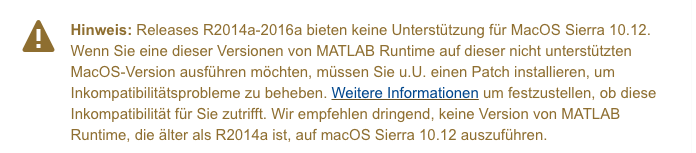
\includegraphics[width=0.9\linewidth]{img/hinweis.png}
\caption{Requirements}
\label{fig:req1}
\end{figure}

However, after setting up those requirements the folder is not created where it should be after the installation is run.
\begin{figure}
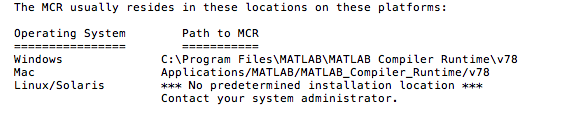
\includegraphics[width=0.9\linewidth]{img/pathShould.png}
\caption{Tuning with SPOT}
\label{fig:tune2}
\end{figure}

It is created here:
\begin{figure}
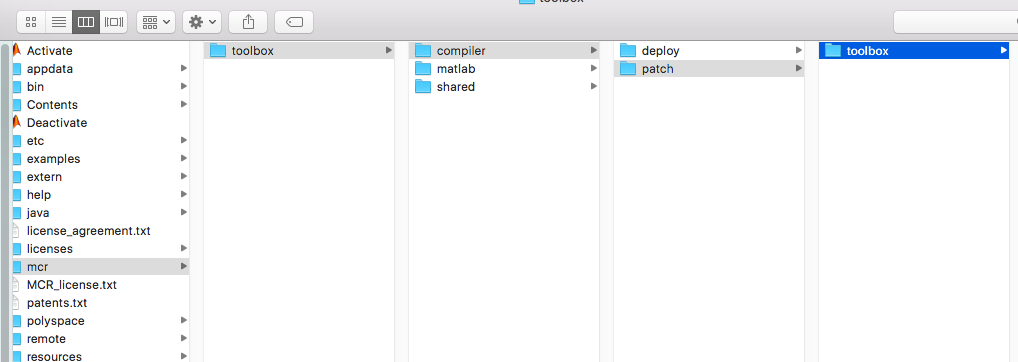
\includegraphics[width=0.9\linewidth]{img/mcrPath.png}
\caption{Tuning with SPOT}
\label{fig:tune2}
\end{figure}

Working with only the matlab files without this causes the following name error:

\begin{figure}
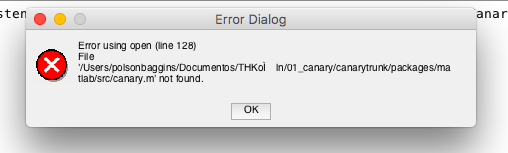
\includegraphics[width=0.9\linewidth]{img/errorName.png}
\caption{Tuning with SPOT}
\label{fig:tune2}
\end{figure}

Which was solved changing the folder name.

\begin{figure}
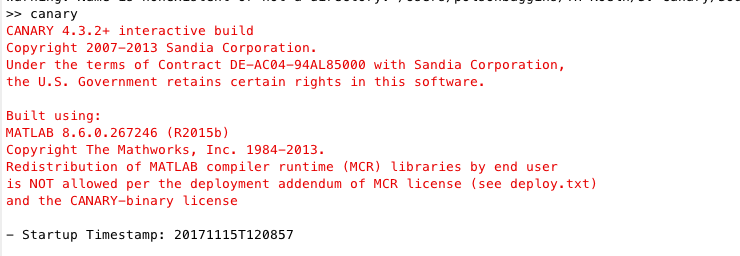
\includegraphics[width=0.9\linewidth]{img/error1.png}
\caption{Tuning with SPOT}
\label{fig:tune2}
\end{figure}

\begin{figure}
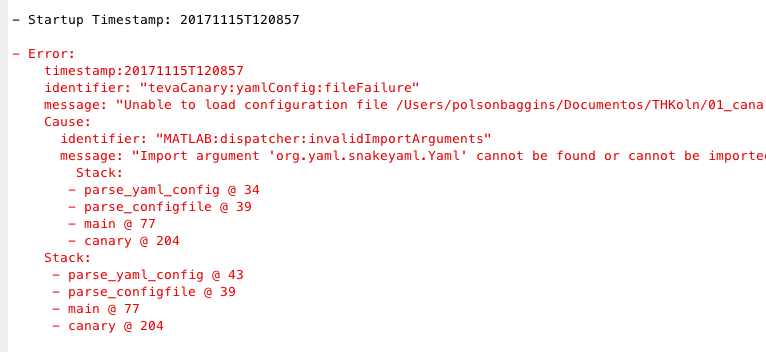
\includegraphics[width=0.9\linewidth]{img/error2.png}
\caption{Tuning with SPOT}
\label{fig:tune2}
\end{figure}

Section~\ref{sec:rev} introduces TSP.
Section~\ref{sec:imp} describes Simulated Annealing.


\section{Introduction }\label{sec:sann}
\section{Review of CANARY and its features }\label{sec:rev}
\section{Introduction to Octave }\label{sec:intr}
\section{Your implementation description  }\label{sec:imp}
\section{Performance measures  }\label{sec:permes}
\section{Testbed }\label{sec:test}
\section{Comparison of performances  }\label{sec:test}
\section{Results and Conclusion }\label{sec:test}
\subsection{The Algorithm}

\subsection{Implementation in R}

\section{Sequential Parameter Optimization}
\subsection{Overview}
 The SPOT package can be installed from within R using the 
\begin{verbatim}
install.packages("SPOT")
\end{verbatim}
command. Alternatively, SPOT can 
downloaded from the
comprehensive R  archive network at \url{http://CRAN.R-project.org/package=SPOT}.
The latter procedure is recommended for the experienced R user only. 
SPOT is one possible implementation of the \emph{sequential parameter optimization}\/
(SPO) framework introduced in~\cite{Bart06a}.
For a detailed documentation of the functions from the SPOT package, the
reader is referred to the package help manuals.
\cite{Bart12i} introduces the SPOT and applications.
\subsection{Interfacing With Simulated Annealing}
In Figure~\ref{fig:tune2} the tuning is shown.


%\begin{figure}
%\includegraphics[width=0.9\linewidth]{cnt0015Ackley83.pdf}
%\caption{Tuning with SPOT}
%\label{fig:tune2}
%\end{figure}

\section{Experiments}

\section{Results}

\section{Discussion}

\section{Summary}
Knuth says:
\cite{knuth2005art}

\bibliographystyle{splncs03}
\bibliography{ReportSample}

\end{document}